\documentclass{article}
\usepackage{tikz}
\usetikzlibrary{positioning}

\begin{document}

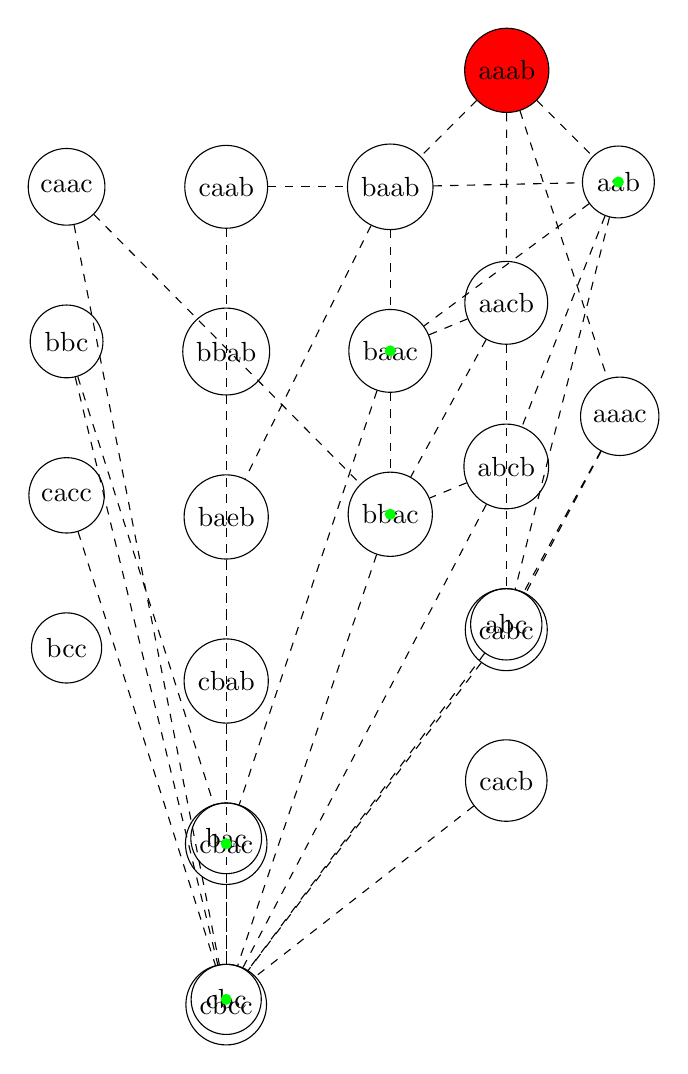
\begin{tikzpicture}[node distance=1cm]
    % Define nodes
    \node (aaab) [circle, draw, fill=red] {aaab};
    \node (baab) [circle, draw, below left=of aaab] {baab};
    \node (aab)  [circle, draw, below right=of aaab] {aab};
    \node (aacb) [circle, draw, below right=of baab] {aacb};
    \node (aaac) [circle, draw, below right=of aacb] {aaac};
    \node (caab) [circle, draw, left=of baab] {caab};
    \node (bbab) [circle, draw, below=of caab] {bbab};
    \node (baeb) [circle, draw, below=of bbab] {baeb};
    \node (baac) [circle, draw, below=of baab] {baac};
    \node (abcb) [circle, draw, below=of aacb] {abcb};
    \node (abc)  [circle, draw, below=of abcb] {abc};
    \node (caac) [circle, draw, left=of caab] {caac};
    \node (bbc)  [circle, draw, below=of caac] {bbc};
    \node (cbab) [circle, draw, below=of baeb] {cbab};
    \node (bbac) [circle, draw, below=of baac] {bbac};
    \node (cabc) [circle, draw, below=of abcb] {cabc};
    \node (cacb) [circle, draw, below=of abc] {cacb};
    \node (bac)  [circle, draw, below=of cbab] {bac};
    \node (cacc) [circle, draw, below=of bbc] {cacc};
    \node (cbac) [circle, draw, below=of cbab] {cbac};
    \node (cbc)  [circle, draw, below=of cbac] {cbc};
    \node (bcc)  [circle, draw, below=of cacc] {bcc};
    \node (cbcc) [circle, draw, below=of cbac] {cbcc};

    % Draw edges
    \draw[dashed] (aaab) -- (baab);
    \draw[dashed] (aaab) -- (aab);
    \draw[dashed] (aaab) -- (aacb);
    \draw[dashed] (aaab) -- (aaac);
    \draw[dashed] (baab) -- (aab);
    \draw[dashed] (baab) -- (baac);
    \draw[dashed] (baab) -- (baeb);
    \draw[dashed] (aab) -- (baac);
    \draw[dashed] (aab) -- (abcb);
    \draw[dashed] (aab) -- (abc);
    \draw[dashed] (aacb) -- (baac);
    \draw[dashed] (aacb) -- (bbac);
    \draw[dashed] (aacb) -- (cabc);
    \draw[dashed] (aaac) -- (aaac);
    \draw[dashed] (aaac) -- (abc);
    \draw[dashed] (aaac) -- (cabc);
    \draw[dashed] (caab) -- (baab);
    \draw[dashed] (caab) -- (bbab);
    \draw[dashed] (caab) -- (cbab);
    \draw[dashed] (bbab) -- (baeb);
    \draw[dashed] (bbab) -- (cbab);
    \draw[dashed] (baeb) -- (cbab);
    \draw[dashed] (baeb) -- (cbac);
    \draw[dashed] (baac) -- (bbac);
    \draw[dashed] (baac) -- (cbac);
    \draw[dashed] (abcb) -- (bbac);
    \draw[dashed] (abcb) -- (cbc);
    \draw[dashed] (abc) -- (cbc);
    \draw[dashed] (caac) -- (bbac);
    \draw[dashed] (caac) -- (cbc);
    \draw[dashed] (bbc) -- (cbac);
    \draw[dashed] (bbc) -- (cbc);
    \draw[dashed] (cbab) -- (cbac);
    \draw[dashed] (cbab) -- (cbc);
    \draw[dashed] (bbac) -- (cbc);
    \draw[dashed] (cabc) -- (cbc);
    \draw[dashed] (cacb) -- (cbc);
    \draw[dashed] (bac) -- (cbac);
    \draw[dashed] (bac) -- (cbc);
    \draw[dashed] (cacc) -- (cbc);
    \draw[dashed] (cbac) -- (cbc);
    \draw[dashed] (cbc) -- (cbc);

    % Color some nodes
    \fill[green] (aab) circle (2pt);
    \fill[green] (baac) circle (2pt);
    \fill[green] (bbac) circle (2pt);
    \fill[green] (cbac) circle (2pt);
    \fill[green] (cbc) circle (2pt);
\end{tikzpicture}

\end{document}